
\section{Introdução}
Elevadores são dispositivos que estão presentes na maioria dos edifícios, sendo em muitos casos essenciais para o acesso das pessoas aos andares mais elevados. Um elevador, de forma genérica, possui sensores (botões de cada andar, sensores de posição) e atuadores (motor de subida/descida, motor das portas e luzes dos botões de andar).

Este projeto tem o objetivo de desenvolver um controlador de elevador com o Kit LPC1768, usando o sistema operacional CMSIS-RTOS. O controlador será responsável por gerenciar todos os aspectos da lógica de funcionamento do elevador.

\section{Objeto}
O produto tem o propósito de ser um controlador de elevador, recebendo requisições de usuários nos botões de cada andar e nos botões internos, e efetuando o controle dos atuadores (luzes de botões, motor de subida/descida e portas) conforme essas requisições. De forma eficiente, o elevador deve atender às demandas dos usuários.

\section{Domínio do problema}

Para o gerenciamento de um elevador, há aspectos importantes que devem ser observados com relação ao seu funcionamento.  O elevador possui limitações quando à sua aceleração máxima. Portanto, há um intervalo mínimo de tempo para ele conseguir parar quando recebe uma requisição de um usuário. De forma mais detalhada, estas limitações temporais estão expostas na seção \ref{sec:espec_nao_funcional}.
% Especificamente, no caso do elevador (simulado) deste projeto, o elevador tem em média no máximo 40 ms para atender a uma requisição 

Com relação à segurança, as portas somente devem ser abertas quando o elevador está parado em algum andar (posicionado dentro de uma faixa de segurança). Também, o elevador só deve mover-se com as portas fechadas.


% \subsection{Segurança}
% A segurança é um fator primordial, que, dentro do contexto deste projeto, envolve o gerenciamento correto dos motores do elevador (subida/descida e portas). Primeiramente, deve-se notar os fatores físicos 

\section{Contexto}

A Figura \ref{fig:diagrama_blocos} apresenta o diagrama de blocos com uma visão geral do sistema. Um computador executa continuamente uma simulação de elevador. O usuário interage diretamente com esta simulação através do mouse, pressionando botões (internos e externos) do elevador. O Kit LPC1768 faz o papel de controlador do elevador, gerenciando a lógica de movimentação e de abertura/fechamento de portas. O Kit e o computador comunicam-se via interface serial, sendo que o Kit controla o comportamento do elevador na simulação, e o computador envia ao Kit comandos de botões do usuário. 

\begin{figure}[h]
    \centering
    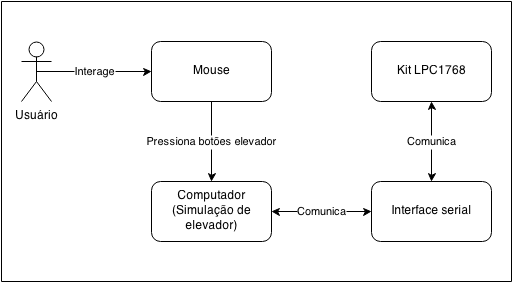
\includegraphics[width=0.8\columnwidth]{./figures/diagrama_blocos.png}
    \caption{Diagrama de blocos do sistema.}
    \label{fig:diagrama_blocos}
\end{figure}


\section{Interfaces}
[TODO: INSERIR FIGURA DO SIMULADOR]

\subsection{Comunicação serial}
O computador (executando a simulação de elevador) e o Kit LPC1768 se comunicarão através de uma interface serial. Os dados serão transmitidos a uma taxa de 115200 bits por segundo. A transmissão, recepção e interpretação dos dados (em ambos os lados) será feita com caracteres ASCII.


\section{Especificação funcional}
\label{sec:espec_funcional}



Os requisitos funcionais levantados para o \it{software} são:

\begin{enumerate}[label=RF \arabic*. , ref=\arabic*]
	\item O sistema deverá ligar a luz de um botão quando este for pressionado.
  \item O sistema deverá desligar a luz de um botão quando o elevador parar no andar correspondente ao botão.
  \item O sistema deverá abrir as portas quando o elevador parar em um andar.
  \item O sistema deverá impedir que as portas sejam abertas quando o elevador não estiver posicionado em um andar.
  \item O sistema deverá impedir que as portas sejam abertas quando o elevador estiver em movimento.
  \item O sistema deverá impedir que o elevador se movimente quando as portas estiverem abertas.
  \item O sistema deverá atender a requisições de andar, feitas através dos botões internos e externos.
  \begin{enumerate}[label*=\arabic*.]
    \item O sistema deverá manter a direção de seu movimento (subida/descida) atual, atendendo todas as requisições que estejam no trajeto.
    \begin{enumerate}[label*=\arabic*.]
        \item O sistema deverá parar o elevador quando ele estiver passando por um andar que o botão interno correspondente tenha sido pressionado.
        \item O sistema deverá parar o elevador quando ele estiver passando por um andar que o botão externo tenha sido pressionado, se estiver indo na mesma direção que a requisição foi feita.
    \end{enumerate}
    \item O sistema deverá inverter a direção de movimento (subida/descida) se houverem requisições na direção contrária, porém somente quando tiver atendido a todas as requisições do trajeto atual.
  \end{enumerate}
  \item O sistema deverá manter o elevador parado no andar atual quando não houverem requisições pendentes.
%   \item O sistema deverá fechar as portas do elevador quando ele estiver ocioso (sem requisições pendentes).
  \item O sistema deverá esperar no mínimo 5 segundos após as portas terem sido abertas antes de fechá-las novamente.
  \item O sistema deverá esperar meio segundo após fechar as portas antes de deslocar o elevador.
  \item O sistema deverá esperar meio segundo após o elevador parar antes de abrir as portas.
%   \item O sistema deverá esperar no mínimo 2 segundos para fechar a porta após um botão interno ser pressionado.
\end{enumerate}

\section{Especificação não-funcional}
\label{sec:espec_nao_funcional}

Os requisitos não-funcionais levantados para o \it{software} são:

\begin{enumerate}[label=RNF \arabic*. , ref=\arabic*]
  \item O sistema deverá parar o elevador após chegar no andar em no máximo 40 milissegundos.
  \item O sistema deverá responder a uma requisição em no máximo 40 milissegundos.
  \item O sistema deverá acender a luz correspondente em no máximo 10 milissegundos após um botão ter sido pressionado.
\end{enumerate}








